\documentclass[]{report}

\usepackage{amsmath}
\usepackage{amssymb}
\usepackage{amsfonts}
\usepackage{cleveref}
\usepackage{verbatim}
\usepackage{listings}
\lstset{basicstyle=\footnotesize\ttfamily, breaklines=true, frame=single, captionpos=b, tabsize=2,upquote=true}
\crefname{lstlisting}{listing}{listings}
\Crefname{lstlisting}{Listing}{Listings}
\usepackage{graphicx}
\usepackage{dirtree}

\usepackage{todonotes}

%Bibliography.
\usepackage[backend=biber]{biblatex}
\addbibresource{references.bib}

%Type setting for numbering.
%\setcounter{tocdepth}{3}
%\setcounter{secnumdepth}{3}

% Title Page
\title{$\mathcal{S}$ide-channel $\mathcal{M}$atters: a $\mathcal{U}$niversal po$\mathcal{R}$table $\mathcal{F}$ramework\\ The \smurf Library}
\author{Yan Yan}

\providecommand{\smurf}{$\mathcal{SMURF}\;$}
\providecommand{\uelmo}{$\mu$-ELMO}
\providecommand{\xor}{\oplus}
\providecommand{\lquote}{\text{`}}
\providecommand{\rquote}{\text{'}}
\providecommand{\ldquote}{\text{``}}
\providecommand{\rdquote}{\text{''}}

%\newenvironment{Ccode}{{\begin{lstlisting}[language=C++]}\\}{{\end{lstlisting}}}
\providecommand{\args}[1]{{\ttfamily{#1}}}
\providecommand{\api}[1]{\paragraph{#1}}

\providecommand{\cmark}{\checkmark}
\providecommand{\xmark}{$\times$}

\providecommand{\yynote}[1]{\todo[backgroundcolor=white]{\color{red} #1}}

\providecommand{\SMURFSUCCESS}{\args{SMURF\_SUCCESS}}
\providecommand{\SMURFERROR}{\args{SMURF\_ERROR}}

\begin{document}
\maketitle

\begin{abstract}
	\smurf is a framework/library for leakage simulator development.
\end{abstract}


\tableofcontents


\chapter{Introduction}


\begin{comment}
\section{An overview: designing a crypto device}
Designing a cryptographic device with side channel awareness is complex. The procedure involves certain roles and the processes:
\begin{itemize}
	\item The \textbf{Hardware designer} designs the hardware with Hardware Design Languages (HDL) such as VHDL or Verilog, and then
	\item the \textbf{Software developer} provides the cryptographic software that would be executed on the device.
	\item Finally the \textbf{side channel Analysts} evaluates the potential leakages of the implementation that has both hardware and software integrated.
\end{itemize}

Several iterations of the procedure are needed alongside revisions. However, participants of different roles each requires a highly dedicated set of skills and are working in very different technical terminologies. As such, bridging the participants is vital yet it can rarely be found suitable candidates that are capable to have coverage over such a wide field of knowledge in reality. This contradiction has grown over the years becoming one of the most significant obstacle among the industry.
\end{comment}

\section{Leakage simulator}
Leakage simulators are simulators enhanced with the functionality of producing leakage traces. They take as input cryptographic implementations cross compiled into binary images on the target platforms, and output leakage traces by applying artificial leakage models to the simulation.

%[Pros and cons]
Leakage simulators are very useful tools for early stage side channel evaluations as an alternative to real devices. Specifically, they have the advantages of:
\begin{itemize} %Pros
	\item \textbf{Low cost} There is no need for real hardware and thus the manufacturing cost are saved. It also made it possible for massive leakage trace generation in parallel, as much as the computational power is affordable.
	\item \textbf{Flexibility} The users can customise the leakage simulator according to the needs, particularly when the leakage simulator is open sourced. For instance, it may allow any chosen fault to be injected at any point during the execution which, in contrast, is very difficult and costly to be achieve on real devices.
	\item \textbf{Better explanatory} Since the leakage are simulated its components can be broken down easily under a known leakage model. This particularly useful in analysing the causes when leakages are detected. This is rather a difficult task for real devices due to physical constrains including synchronisation and measurement errors, especially under a non invasive setting.
\end{itemize}

%Cons
On the other hand, it must be noted that leakage simulator has its constrains. Above all, the quality of a leakage simulator is determined by the quality of the leakage model it employed, which is often judged by its representativeness towards physical devices. Hence certain degree of error is inevitable and it is an active research topic improving the modelling methods to mitigate such error. In reality, leakage simulators also must face the problem black box modelling, i.e. the leakage models are modelled by third parties that does not necessarily have access to the exact hardware design. This is typically seen on commercial products since their hardware designs are often propitiatory.


\paragraph{Examples of leakage simulator}
A simplest example is the Hamming weight simulators which are frequently seen in side channel literatures. Its leakage at each time point is simulated simply by summing the Hamming weights of all operands. The popularity of Hamming weight could be traced back to the earliest side channel literatures such as ~\cite{CPA} due to its empirical successful application on real devices and it has lasted even until today. Alternatively, Hamming distance has also been used in a similar manner when people trying to capture transitional leakage between two intermediates~\cite{CPA}.

However, as the semiconductor technology evolves over the decades, Hamming weight can now hardly be seen as a well captured leakage model for the latest devices. Particularly due to the fact that none of the microarchitecture factors has been taken into account in the Hamming weight model whereas in reality they have been shown to be significantly contributing to the leakage. The ELMO~\cite{ELMO} project is a remarkable example that addressed this issue by introducing an abstracted ELMO architecture that consists an ALU and pipeline. The ELMO architecture enables the leakage to be depicted with a better granularity since the leakage model is taking more detailed intermediates rather than simply the operands. ELMO also proposed the idea of depicting the leakage model as a linear function of the intermediates with coefficients derived from regressing the real traces. As a result, ELMO traces are more realistic and hence better leakage coverage than simply Hamming weight and Hamming distances. ELMO has later spawned the GILES\cite{GILES} which additionally supports fault injection.

A further step down the line is the \uelmo project~\cite{SiModel,SiReverse}. Comparing with its predecessor, \uelmo is built on a more realistic architecture rather than an abstraction as did by ELMO which allows leakage model to be defined with further realisticness. Since more intermediates are captured during the simulation, \uelmo also creates a better potential of portability for the proving tools used by provable side channel analysis (more details in \Cref{sec:ProvableSCA}). However, there are certain practicability flaws in \uelmo. First of all, having access to the architectural information is generally a difficult task, especially for commercial products where the designs are proprietary. Secondly, it is also practically difficult to include every component in a processor into the leakage model due to its complexity. In case of \uelmo, the architecture was derived from reverse engineering the device~\cite{SiReverse} and then a selection process (details in \cite{SiModel}) is needed to produce a set of architectural components that are significant to leakage. 

%[Other leakage simulators.]

\section{Provable side channel and the proving tools\label{sec:ProvableSCA}}
[I need input from Ines on this topic...]


\section{The \smurf solution}
\subsection{History: from ELMO to \uelmo}
The initiative of \smurf stems from the ELMO~\cite{ELMO} project. The goal was to provide a proof of concept for building a more sophisticated leakage simulator that captures architectural leakage context. The code was developed based on the open sourced Thumbulator~\cite{Thumbulator}. As a prototype of its kind, ELMO nicely simulated the leakage of its targeted device which is an ARM Cortex-M0 on a STM32F0 board.

The ELMO leakage simulator has later been restructured into GILES~\cite{GILES}, which additionally supported fault injection simulation. The decision to restructure ELMO was made due to the fact that the code was highly entangled with Thumbulator and lack comprehensible extensibility. The restructured GILES takes a configuration file in JSON format for coefficients in the leakage model which was hardcoded in the original ELMO. Also as a side project, GILES additionally provides the functionality of fault injection simulation.

Although GILES was intended to have a generic framework that could be reused for further development of other leakage simulators, it was later found unsatisfactorily meeting this expectation in the \uelmo project. Firstly, GILES is written in C++ and its interface to other emulators has been designed at the code level, that is, to reuse the GILES framework the developer is required to integrate the source code of the emulator into GILES code base and then recompile the integrated code to generate the executable.  As a generic solution, such design could be problematic in certain scenarios, e.g. developers might need to solve problems caused by cross compiling when the emulator is not written in C/C++, and/or part of the emulator must be adapted to be compatible to GILES' code interface. Secondly, GIELS' interface are defined based on the abstracted ELMO architecture. This directly caused the GILES' framework being abandoned during the development of \uelmo, since it is based on a realistic architecture that is not compatible with ELMO's.

\subsection{The \smurf framework}
Reviewing the predecessors, it does not take long to conclude that there is a great engineering difficulty in implementing a leakage simulator platform that can invoke a third party emulator and apply a customisable leakage model to generate leakage traces in a comprehensive manner. Therefore comes the idea of \smurf: rather than plugging different components into a generic leakage simulator platform as attempted in GILES, \smurf inverts the approach by being a ``middleware''. That is, it is designated to be a library that is serves as a plugin to different components providing a data exchanging mechanism.

\smurf focuses on two major tasks during the life cycle of a leakage simulator:
\begin{itemize}
	\item \smurf  provides an universal interface to the emulator for exporting execution traces, i.e. execution details such as states of registers, flags and buses during the emulation. The Execution Traces are store in a portable format. The execution traces are combined with the measured traces from real devices to deduce the leakage model, which then to be integrated into the leakage simulator. Finally the simulated leakage traces are generated for vulnerability evaluation where \smurf can help porting information from the emulator to the leakage simulator.
	
	\item \smurf also provides a set of universal interfaces for the leakage simulator to interact with the proving tools. Firstly, it provides an interface of instructing the leakage simulator to annotate the simulated traces with symbolic information. Secondly, it provides the functionality to export the symbolic traces, i.e. the simulated traces with annotated symbolic information, that can later be imported to proving tools in the back end with \smurf.
\end{itemize}

In the technical aspect, the \smurf design prioritises portability and modularity. \Cref{fig:Overview} summaries the framework.

\begin{figure}
	\centering
	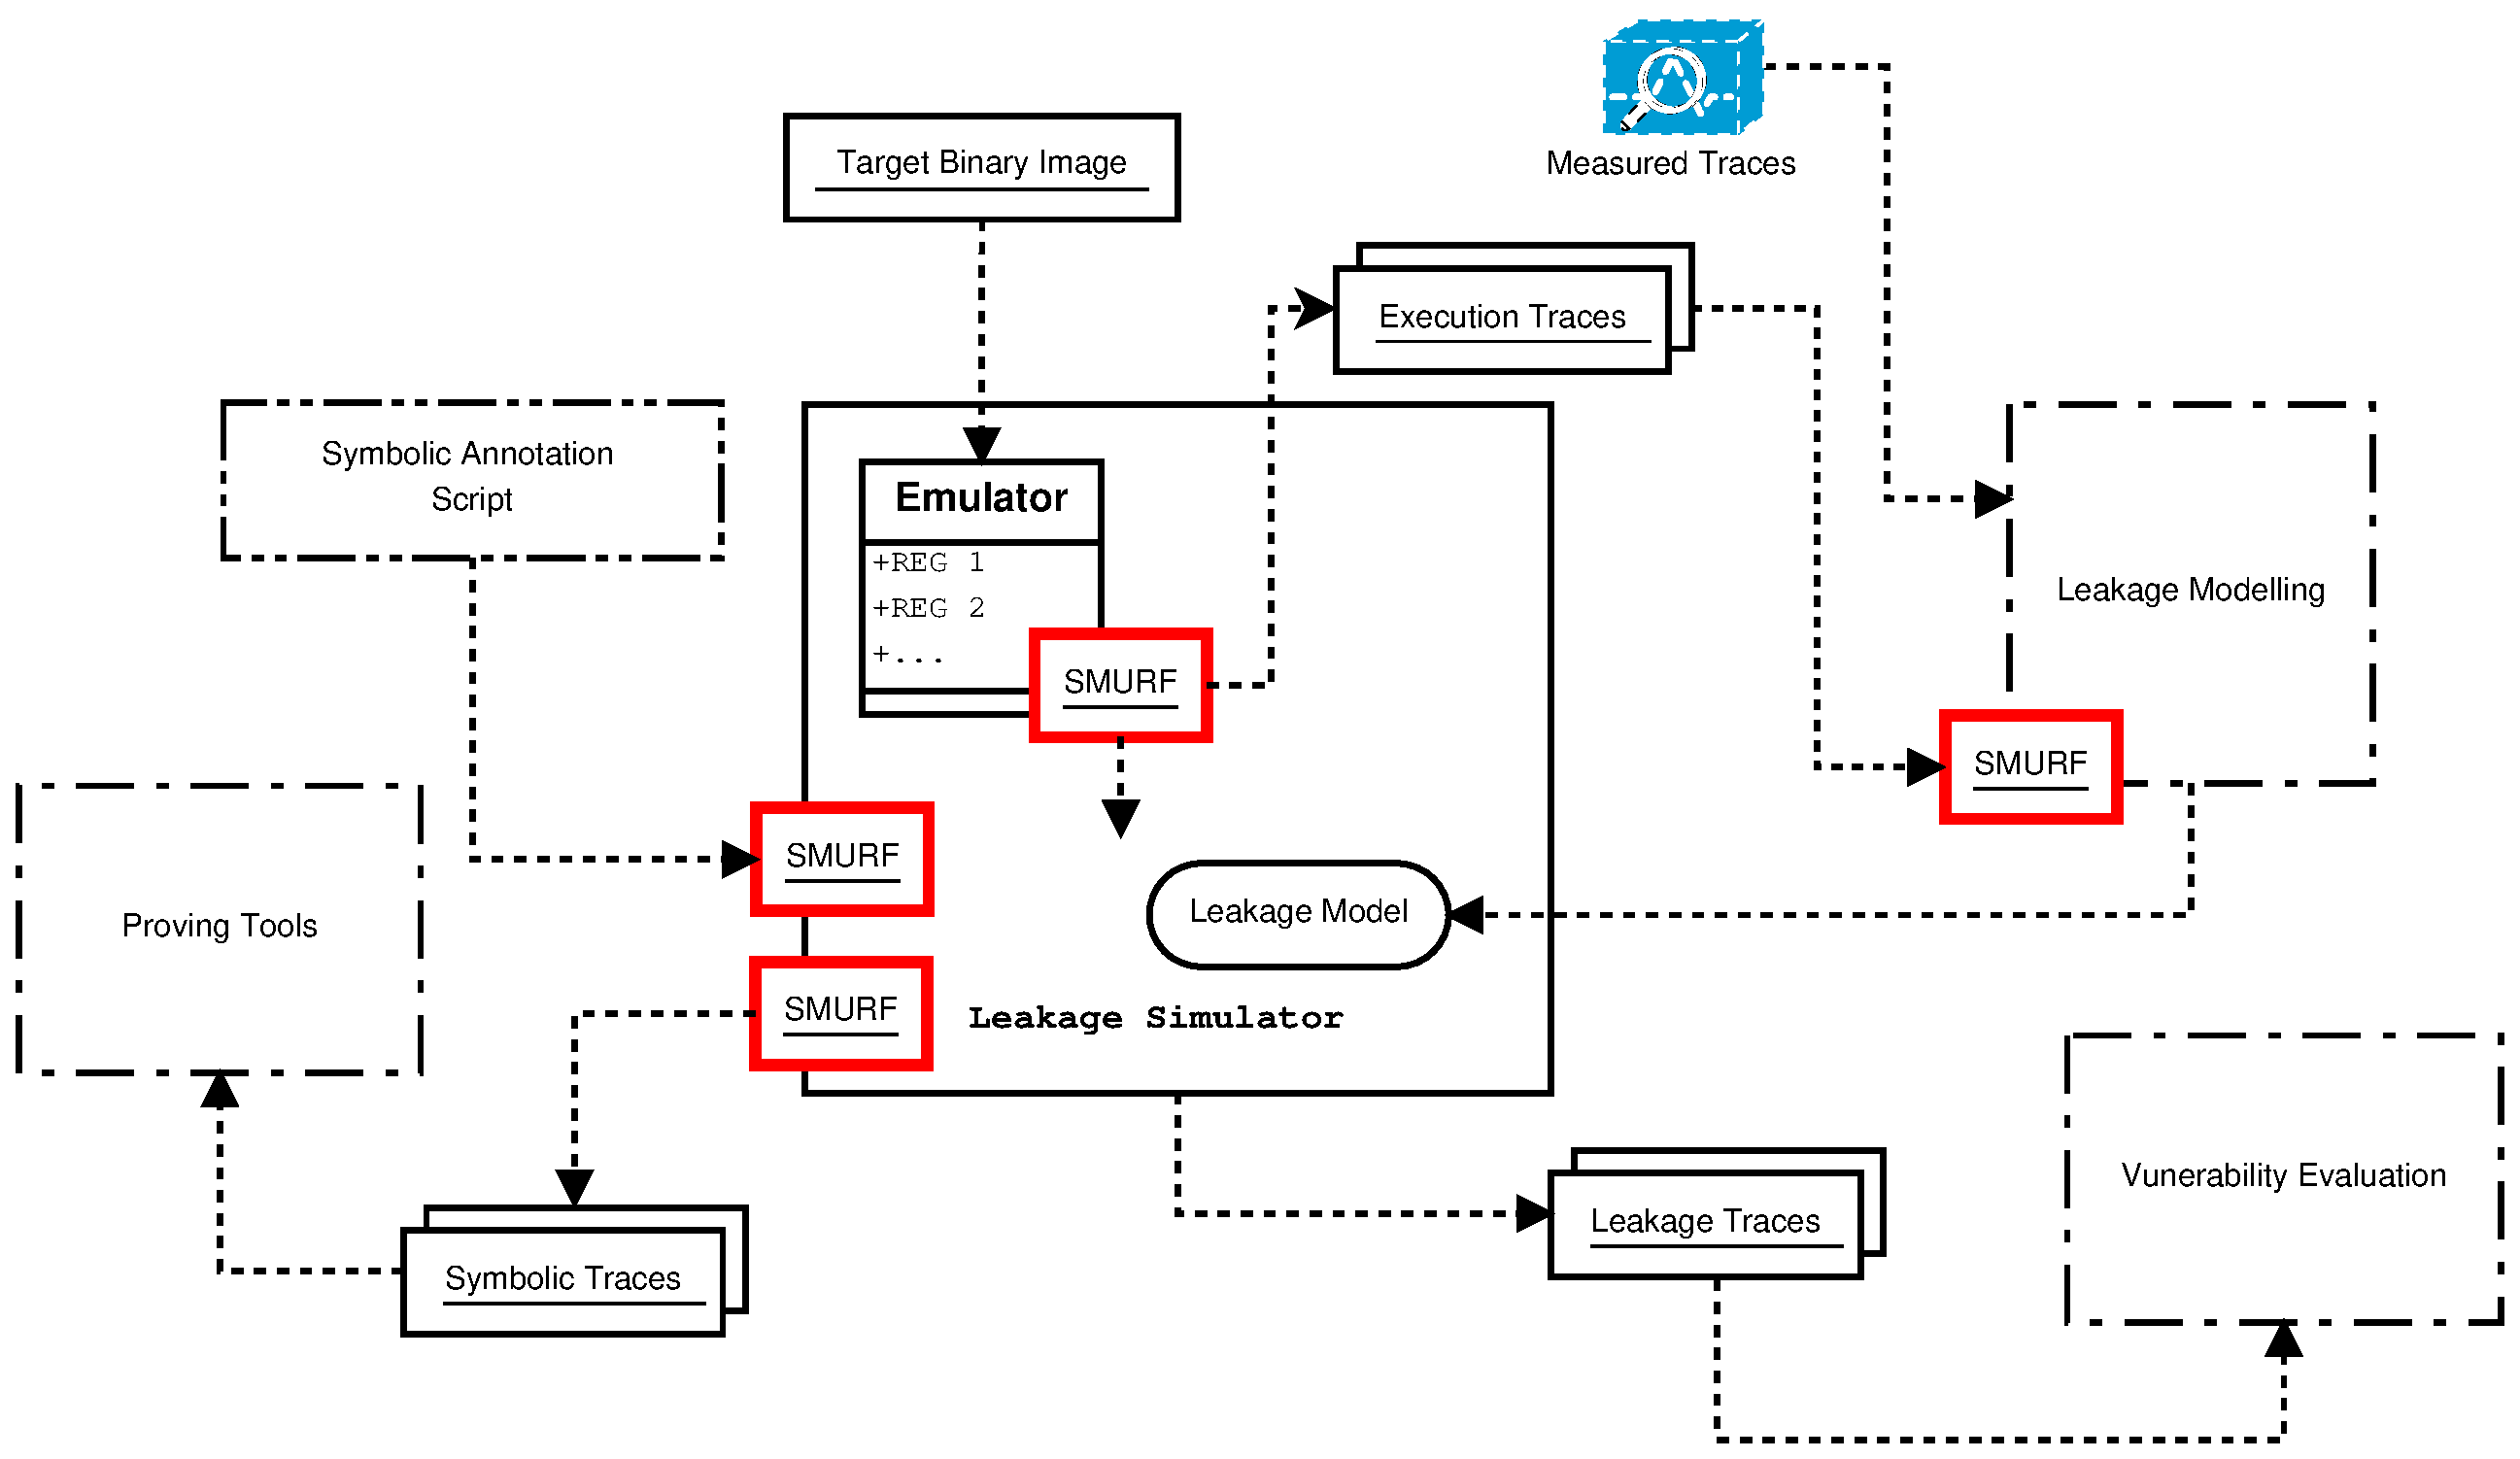
\includegraphics[width=0.9\linewidth]{./Figures/Overview.eps}
	\caption{An Overview of \smurf \label{fig:Overview}}
\end{figure}


\chapter{User's Manual}
\section{Introduction}
The design of \smurf follows the concept of Object Oriented and is highly modularised. C/C++ and Python3 are chosen as the supported languages for their generic usage in emulator development and data analysis. The library is written fully compatible with POSIX.1-2001~\cite{POSIX} standard for best portability among various UNIX-style operating systems.

\section{\smurf objects\label{sec:SmurfObjects}}
We first introduce the major objects within the \smurf framework.

\subsection{Core}
The Core object is the abstraction of the target device to be simulated. A Core is constituted of multiple Components (see below) representing either physical components in the hardware or abstracted attributes of the device.

\subsection{Component}
The Component objects are the objects that describe the Core. For comprehensiveness, they can be categorised into two categories:
\begin{itemize}
	\item Physical Components. These represents physically existed components within the device such as registers, flags or buses.
	\item Virtual Components. They are used to represent arributes of the Core which does not have a correspondence physically. Some examples in this category are time in the simulation, or human readable descriptions in fetching, decoding and execution cycles. They may also be used to represent tuples of other Components, such as ``(Reg1, Reg2)'' which could be used in scenarios like multivariate leakage analysis.
\end{itemize}

The state of a Component is described by four attributes, namely name, type, length and value. Most of the Component types have their equivalence in C99. Static\footnote{a.k.a fixed length} array declaration is supported except for the STRING type, where the lenght of array\footnote{a.k.a. number of elements} is indicated by the Component length. For STRING type Component, only strings of ASCII characters are accepted as the value and the length indicates the maximum number of characters including the NULL terminator `$\backslash 0$'. A reference table is given in \Cref{tbl:ComponentTypes}.

\begin{table}
	\centering
	\begin{tabular}{|c|c|l|}
	\hline
	Component Type & Reference C99 data type & \multicolumn{1}{c|}{Note}                                                                                                                               \\ \hline
	BOOL       & bool                    &                                                                                                                                                         \\ \hline
	OCTET      & uint8\_t                &                                                                                                                                                         \\ \hline
	STRING     & char *                  & \begin{tabular}[c]{@{}l@{}}Only ASCII strings.\\ No array support.\\ Length: max \# of characters (including $\backslash 0$).\end{tabular} \\ \hline
	INT16      & int16\_t                &                                                                                                                                                         \\ \hline
	UINT16     & uint16\_t               &                                                                                                                                                         \\ \hline
	INT32      & int32\_t                &                                                                                                                                                         \\ \hline
	UINT32     & uint32\_t               &                                                                                                                                                         \\ \hline
\end{tabular}
	\caption{Smurf Component Types\label{tbl:ComponentTypes}}
\end{table}

\Cref{fig:CoreAndComponents} shows an example of a Core containing several Components.

\begin{figure}
	\centering
	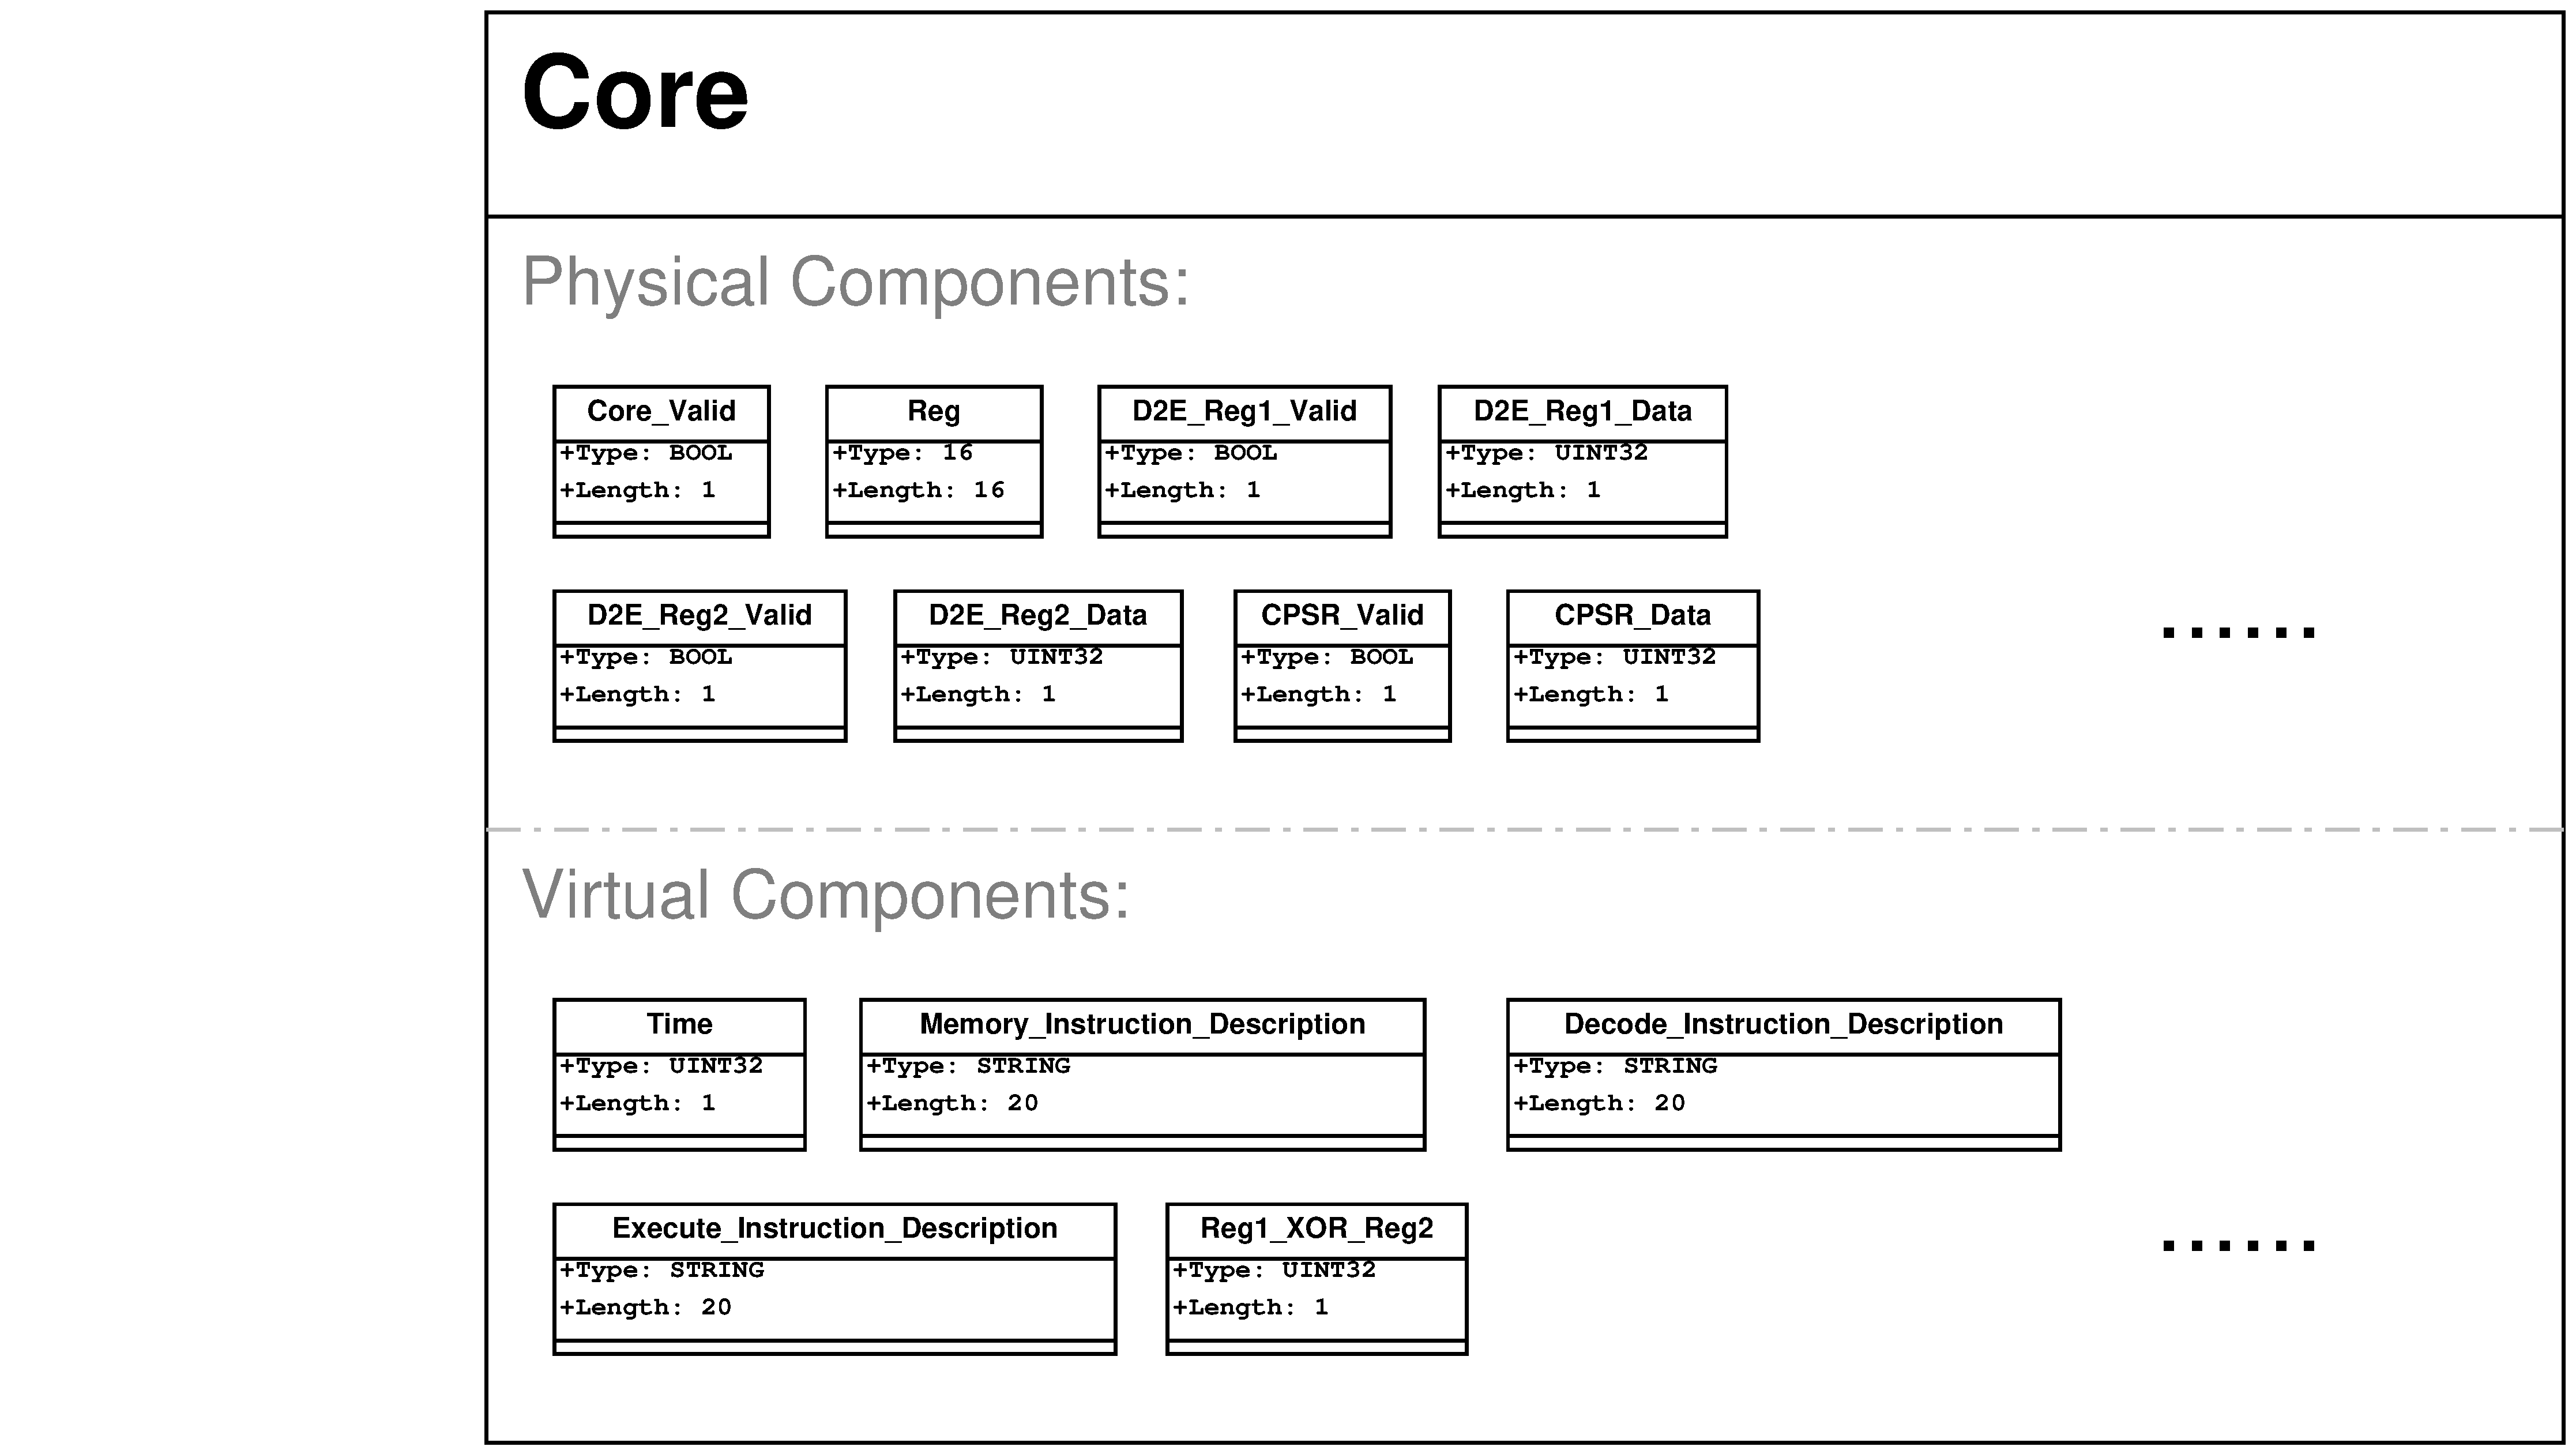
\includegraphics[width=0.8\linewidth]{Figures/Core.eps}
	\caption{Example of Core and Components\label{fig:CoreAndComponents}}
\end{figure}

\subsection{Trace}
The Trace object is a sequence of Frames (see below) that records the simulation. In the \smurf framework it is the major outcome of emulation and simulation and may adopt different forms depending on the usage (e.g. to have execution details in the Execution Trace, symbolic information in the Symbolic Trace, or be applied a leakage model in the Leakage Trace).

\subsection{Frame}
A Frame is a record of the state of Core at a specific moment during the simulation. A Frame can be considered an instantiated Core where values are assigned to its Components at the moment of being record. We refer to this valued Components in a Frame as Component Instances.

An important note is that the \smurf framework does not specify at which moments during the simulation that a Frame should be recorded and thus it is completely up to the choice of users (i.e. developers of the emulator and the leakage simulator). 

\subsection{Dictionary\yynote{Not finalised yet...} (optional)}
The Dictionary is the collection of all valid Symbols (see below). Note that in contrary to the Core, the Dictionary is dynamic in that it is possible to expand it with new Symbols at the runtime (i.e. during the leakage simulation).

\subsection{Symbol (optional)}
The Symbol objects represent the symbolic representations of intermediate variables during the leakage simulation that are used to generate the Symbolic Traces which are then to be imported by the proving tools. During the simulation, Components in Frames are annotated by Symbols as instructed by a symbolic annotation script specified by the user. 

A Symbol needs to be first declared within Dictionary before it can be annotated by. This can be done at the runtime. \smurf also supports user defined operators over the Symbols, for instance, the user may define an XOR operator:
\[
	\ldquote s_1 \xor s_2 \rdquote := \text{XOR}(\ldquote s_1 \rdquote, \ldquote s_2 \rdquote)
\]
such that it returns a new Symbol ($\ldquote s_1 \xor s_2 \rdquote$) from two Symbols $\ldquote s_1 \rdquote$ and $\ldquote s_2 \rdquote$.

Note that Dictionary and Symbols are optional that are only required if the leakage simulator intends to support the symbolic features. \Cref{fig:TraceAndFrames} gives an example of a Trace of multiple Frames with optional symbolic features.

\begin{figure}
	\centering
	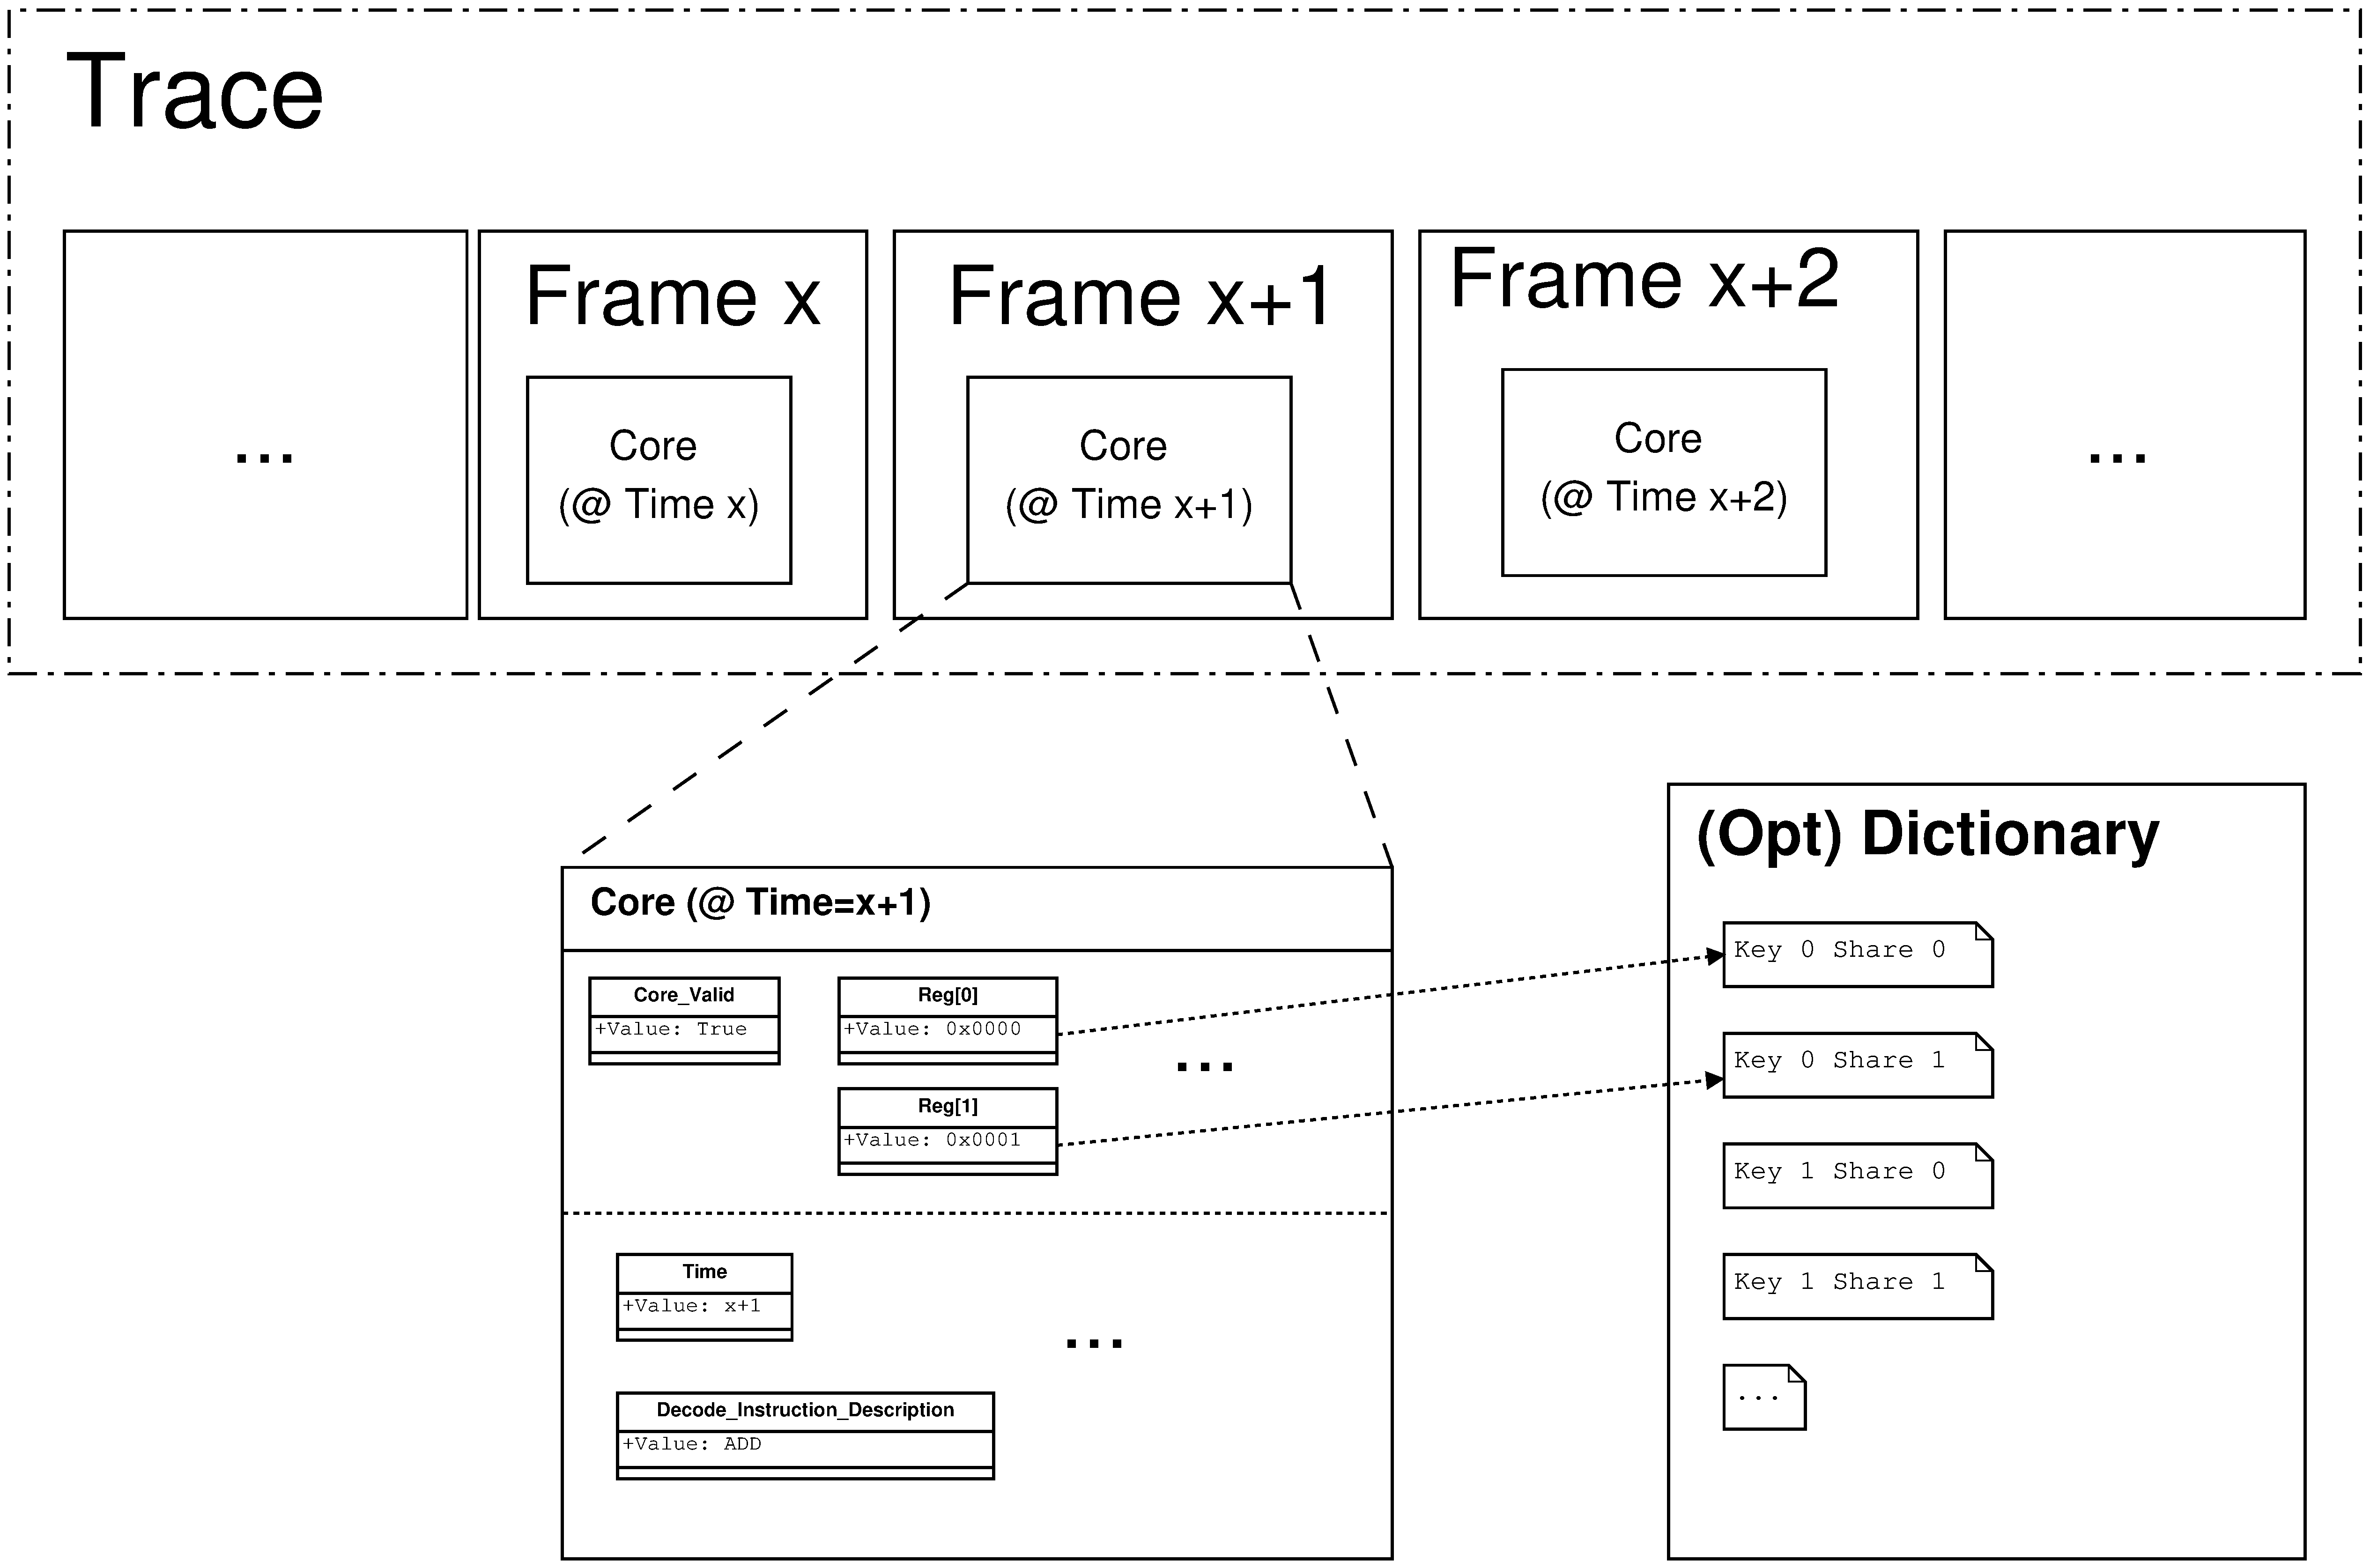
\includegraphics[width=0.9\linewidth]{Figures/Trace.eps}
	\caption{Example of Trace and Frames with Symbolic information\label{fig:TraceAndFrames}}
\end{figure}

A tree view summary of the relationships of \smurf objects is provided in \Cref{fig:SmurfTreeview}.
\begin{figure}
	\dirtree{%
		.1 \_.
			.2 Core.
				.3 [Component](s).
			.2 Trace.
				.3 [Frame](s).
					.4 Core.
						.5 [Component](s) - (Opt)[Symbol](s).
			.2  (Opt) Dictionary.
				.3 (Opt) [Symbol](s) .
	}
	\caption{Tree view of \smurf objects\label{fig:SmurfTreeview}}
\end{figure}

\section{\smurf Modules}
Depending on the theme of functionality, from a high level \smurf can be divided into the following major modules:
\begin{itemize}
	\item The \smurf \textbf{Basic} module provides basic functionalities for manipulating various \smurf objects. Its typical usage include initialising and cleaning of \smurf objects, as well as exporting and importing the \smurf objects into various user programs. APIs within this module are supported both in C/C++ and Python3. 
	
	\item The \smurf \textbf{Emulator} module focuses on tasks related to the emulator, particularly about constructing a \smurf Frame from the internet data structures of the emulator and exporting them as a \smurf Trace to be read by other parties in the \smurf framework. There is also a submodule within this module called SmurfIO that provides an universal interface to simulate a virtual serial port on POSIX compatible systems. This module is supported in C/C++ only as it is designed for the usage of the emulator.
	
	\item \textbf{(Optional)} The \smurf \textbf{Symbolic} module  provides the functionality related to handling symbolic operations. Note that it is implemented as an optional extension that it is up to the decision of leakage simulator to support related features or not. This module is supported both in C/C++ and in Python3.
\end{itemize}

\section{The Smurf Basic module\label{sec:SmurfBasic}}
For C/C++ programs, the corresponding APIs are defined in \args{smurf/smurf.h}. For Python3 programs, the corresponding module is \args{smurf}.

\subsection{Smurf debugging output}
The debugging output of Smurf library are disabled by default. User's can turn it on with \args{SmurfSetVerbose()}:
\begin{lstlisting}[language=C++, caption={SmurfSetVerbose()\label{api:SmurfSetVerboseC}}]
void SmurfSetVerbose(bool dbginfo);

//Turn on debug info.
SmurfSetVerbose(true);

//Turn on debug info.
SmurfSetVerbose(flase);
\end{lstlisting}
Set \args{dbginfo} to \args{true} turns on the debugging output and vice versa.

\subsection{Core specification\label{api:Smurf.Core}}
To begin with the \smurf framework, the first step is to define your Core and generate the Core specification with a Python script. To do so, we first initiate a \args{smurf.Core} object:
\begin{lstlisting}[language=Python,caption={smurf.Core()\label{api:smurf.CoreP}}]
import smurf
	
# Class:
#	smurf.Core()
	
# Example: generate a Core object.
core = smurf.Core()
\end{lstlisting}

Use \args{Smurf.Core.NewComponent()} to add Components into the Core :
\begin{lstlisting}[language=Python,caption={smurf.Core.NewComponent()\label{api:Core.NewComponentP}}]
# Prototype:
#	smurf.Core.NewComponent(compname, comptype='OCTET', complen=1):

# Example: Adding 3 Components "RegA", "RegB" and "RegC".
core.NewComponent("RegA")
core.NewComponent("RegB", 'UINT32')
core.NewComponent("RegC", 'OCTET', 4)
\end{lstlisting}

\args{compname} is the name of the Component given as a string. \args{comptype} is of the types given in \Cref{tbl:ComponentTypes} as a string, and \args{complen} is the size of the Component (in its own type). In the example given in \Cref{api:Core.NewComponentP}, three different Components are added, which are namely:
\begin{itemize}
	\item \args{RegA} that has an ``OCTET'' (8 bit) value, 
	\item \args{RegB} that has an ``UINT32'' (unsigned 32 bit) value, and 
	\item \args{RegC} that has $4$ ``OCTET'' value which in total has $8 * 4 =32$ bits.
\end{itemize}

Once all the Components are added, the Core specification can be dumped into a file using \args{Smurf.Core.Save()}:
\begin{lstlisting}[language=Python,caption={smurf.Core.Save()\label{api:Core.SaveP}}]
# Prototype:
#	smurf.Core.Save(filepath)

# Example: saving the Core into a Core specification
core.Save("./test.core")
\end{lstlisting}

\args{filepath} is the file path of the output Core specification file.

This generates a Core specification file which actually is implemented as a JSON file that can be opened with other viewers such as a browser:
\begin{lstlisting}[caption={test.core\label{test.core}}]
{
	"version": "1",
	"components": {
		"RegA": {
			"type": "OCTET",
			"len": 1
		},
		"RegB": {
			"type": "UINT32",
			"len": 1
		},
		"RegC": {
			"type": "OCTET",
			"len": 4
		}
	}
}
\end{lstlisting}




\subsection{\smurf objects at code level}
\subsubsection{Initialisation and free}
To use the Smurf library in C/C++ programs, a Smurf session must be established first. The APIs are defined in the header ``smurf/smurf.h''.
A Core specification (details in \Cref{api:Smurf.Core}) is required for the initialisation. It is also required that a path of the Trace to be provided during this procedure alongside its mode, which is either read or write. For a reading session, the Core specification is needed to interpret the Trace and for a writing session it determines how data are structured in the Trace. As of a general practice in C/C++ programs, the Smurf session needs to be freed by the end of its lifespam to recycle its resource.

To initialise a Smurf session, use \args{InitSmurf()}:
\begin{lstlisting}[language=C++, caption={InitSmurf()\label{api:InitSmurfC}}]
Smurf* InitSmurf(
const char *corepath, //Path of Core specificatoin.
const char *tracepath, //Path of Trace file.
int tracemode);	//Mode of Trace file.
\end{lstlisting}

The \args{Smurf*} returned by InitSmurf() is the handle of the newly initialised Smurf session. \args{corepath} and \args{tracepath} are the paths of the Core specification and the Trace respectively. There are currently $4$ modes available for the Trace mode argument \args{tracemode}:
\begin{itemize}
	\item To read a Trace, \args{tracemode} should be set to \args{SMURF\_TRACE\_MODE\_READ}.
	\item To write a Trace, \args{tracemode} should be chosen from one of:
	\begin{description}
		\item[\args{SMURF\_TRACE\_MODE\_CREATE}] Creates a new Trace file. The file will be truncated if it already exists.
		\item[\args{SMURF\_TRACE\_MODE\_APPEND}] Opens an existing Trace file and appending new Frames from its end.
		\item[\args{SMURF\_TRACE\_MODE\_FIFO}] Creates a temporary First-In-First-Out (FIFO~\cite{FIFO}) at \args{tracepath}. The FIFO will be removed upon calling \args{FreeSmurf()}.
	\end{description}
\end{itemize}

Notes about the \args{tracemode}:
\begin{itemize}
	\item Trace generated always has been set the permissions of all read and write (i.e. 0666 file mode).
	\item \args{SMURF\_TRACE\_MODE\_READ} is used universaly to read Traces of a regular file (as created with \args{SMURF\_TRACE\_MODE\_CREATE}) or a FIFO (as created with \args{SMURF\_TRACE\_MODE\_FIFO}).
	\item As indicated in POSIX statndard, when calling with \args{SMURF\_TRACE\_MODE\_FIFO}, the process will be blocked until the same FIFO Trace has been opened for read by another process. Behaviours of writing in or reading out the FIFO Trace are also consistent with the FIFO specifications in POSIX.
	\item It is recommend to use \args{SMURF\_TRACE\_MODE\_FIFO} when dealing with exceptionally large Traces, as data written into the FIFO Trace will directly passed to the reader's end by the kernel without going through the harddisk. In constrast, when storage of the Trace is desired, \args{SMURF\_TRACE\_MODE\_CREATE} should be used instead. However, users should be minded that simutaneously reading a regular file Trace as it is being written may create a competition and thus synchronous issues.
\end{itemize}

By the end of the Smurf session, use \args{FreeSmurf()} to free the session:
\begin{lstlisting}[language=C++,caption={FreeSmurf()\label{api:FreeSmurfC}}]
void FreeSmurf(Smurf * smurf);
\end{lstlisting}

\args{FreeSmurf()} has no return value and \args{smurf} is the handle of the Smurf session to be freed, including allocated memory and other system resources such as file descriptors. If args{smurf} is initialised with \args{SMURF\_TRACE\_MODE\_FIFO}, then the associated FIFO Trace will also be deleted.

Once a Smurf session has been initialised, the static \smurf objects described in \Cref{sec:SmurfObjects} can be directly accessed from the user program via data structures within the session \args{smurf}. Note that the structure definitions demonstrated in this section are simplified from the source code such that certain internal data structures are omitted.

For Python3 programs, simply import the \args{smurf} module:
\begin{lstlisting}[language=Python,caption={Importing Smurf module\label{api:ImportSmurfP}}]
	import smurf
\end{lstlisting}

\subsubsection{Core}
The Core is constructed from the Core specification \args{corepath} provided to \args{InitSmurf()}. Core is defined and accessed as:
\begin{lstlisting}[language=C++, caption={struct SmurfCore\label{api:CoreC}}]
typedef struct {
	int ncomponents;	//Number of Core Components.
	SmurfCoreComponent **components;	//Core Components.
} SmurfCore;

//Access.
smurf->core; //Type: SmurfCore*
\end{lstlisting}

Note that \args{smurf->core} is a pointer to the Core object. Within the Core, \args{ncomponents} records the number of Components constitutes the Core and their entries are given as an array of their points. 

In Python3, \args{smurf.Core.Load()} loads a Core specification into a Core object:
\begin{lstlisting}[language=Python,caption={smurf.Core.Load()\label{api:Core.LoadP}}]
# Prototype:
#	smurf.Core.Load(filepath)

# Example: load "test.core".	
core = Smurf.Core.Load("test.core")
\end{lstlisting}
\args{filepath} is the path of the Core specification file to be loaded.

\subsubsection{Component} 
The Components are then defined and accessed as:
\begin{lstlisting}[language=C++, caption={struct SmurfCoreComponent\label{api:ComponentC}}]
typedef struct {
	char *name; //Component name.
	SmurfCoreComponentType type; //Component type.
	size_t len; //Size of Component, measured by its type.
} SmurfCoreComponent;

//Access the i-th Component.
smurf->core->components[i]; //Type: SmurfCoreComponent*
\end{lstlisting}

In particular, the \args{smurf->core->components[i]->type} is one of the following as in \Cref{tbl:ComponentTypes}:
\begin{lstlisting}[language=C++, caption={enum SmurfCoreComponentType\label{api:ComponentTypeC}}]
typedef enum {
	UNDEFINED, 	//Error case.
	BOOL, OCTET, STRING, 
	INT16, UINT16, INT32, UINT32
} SmurfCoreComponentType;
\end{lstlisting}

\args{smurf->core->components[i]->len} is the length of the Component measured by its type. That is, its value is $1$ if the Component has been declared as univariate, or $n$ if the Component has been declared as an array of size $n$. Only for the type \args{STRING}, \args{len} is the maximum number of characters in this Component.

It is important to note that values of Components are not presented within the session \args{smurf} as the data strctures inside \args{smurf} records only the static information. Details of accessing the values of Components are given in \Cref{sec:FrameAPIsC}.

In Python3, the Components are implemented as a dictionary member of the Core. It further has three members namely \args{name}, \args{type} and \args{len}:
\begin{lstlisting}[language=Python,caption={smurf.Core.components\label{api:Core.componentsP}}]
# class:
#	smurf.Core.Component

# Example: print Components in a Core "core"
comps = core.components
for c in comps:
	print("Name:{:s}".format(comps[c].name))
	print("Type:{:s}".format(comps[c].type))
	print("Length:{:d}".format(comps[c].len))
\end{lstlisting}
\args{name} and \args{type} are the name and type of the Component in strings as described in \Cref{sec:SmurfObjects}. \args{len} is the length of the Component in its type(details in \Cref{sec:SmurfObjects}).


\subsubsection{Trace}
Once a Smurf session is initialised, its Trace is opened as a file descriptor in the user's process. Although the relevant resources will be released when the session is freed, the Trace object provides informatoin for management purposes.
\begin{lstlisting}[language=C++, caption={struct SmurfTrace\label{api:TraceC}}]
typedef struct {
	char *path;	//Path of the Trace file.
	int fd;		//File descriptor of Trace file.
	int mode;	//Mode of Trace file as being initialised.
	size_t offset;	//Current Frame offset.
} SmurfTrace;

//Accessing the Trace.
smurf->trace; //Type: SmurfTrace*
\end{lstlisting}

Note that the Trace object should be read only and users should not modify its contents. \args{mode} records the value of \args{tracemode} as being initialised in \Cref{api:InitSmurf}. \args{offset} records the current position of Frame. When the Trace is initialised by \args{SMURF\_TRACE\_MODE\_FIFO}, \args{offset} is effectively the number of Frames read or written.

In Python3, a Trace, \args{smurf.Trace}, needs first be initialised from a Core and then loaded from the file system using \args{smurf.Trace.Open()}. Note that currently in Python3 only Trace reading is supported.
\begin{lstlisting}[language=Python,caption={smurf.Trace\label{api:Core.TraceP}}]
# Class:
#	smurf.Trace

# Example: initialise from "core" and load a Trace at "filepath"
trace = smurf.Trace(core)
trace.Open(filepath)
\end{lstlisting}

\subsubsection{Frame}
The Smurf library implements two types of Frame.

\paragraph{Buffer Frame}
A buffer Frame is allocated alongside session initialisation for quick access:
\begin{lstlisting}[language=C++, caption={struct SmurfFrame\label{api:FrameC}}]
typedef struct {
	int len;	//Size of the Frame in bytes.
	unsigned char *buf;	//Contents of Frame.
} SmurfFrame;

//Accessing the Frame buffer.
smurf->frame; //Type: SmurfFrame*
\end{lstlisting}
Further details of Frame APIs are given in \Cref{sec:FrameAPIsC}.

\paragraph{Self managed Frame}
Alternatively, users may use self managed Frames for more flexibility. To create a self manged Frame within the Smurf session \args{smurf}, use \args{SmurfNewFrame()}:
\begin{lstlisting}[language=C++, caption={SmurfNewFrame()\label{api:SmurfNewFrameC}}]
SmurfFrame *SmurfNewFrame(Smurf * smurf);

//The new self manged Frame newframe:
newframe = SmurfNewFrame(smurf);
\end{lstlisting}
NULL is returned if \args{SmurfNewFrame()} failed.

It lies in the user's responsibility to free the self managed Frames at the end of its lifecycle by calling \args{FreeFrame()}:
\begin{lstlisting}[language=C++, caption={SmurfFreeFrame()\label{api:SmurfFreeFrameC}}]
void *SmurfFreeFrame(SmurfFrame * frame);

//Free the self manged Frame frame:
SmurfFreeFrame(frame);
\end{lstlisting}

\args{CopyFrame()} copies a Frame from one to another:
\begin{lstlisting}[language=C++, caption={CopyFrame()\label{api:CopyFrameC}}]
int *CopyFrame(SmurfFrame * dstframe, SmurfFrame * srcframe);

//Example: copy the buffer Frame into a self manged Frame
SmurfFrame *newframe;
newframe = SmurfNewFrame(smurf);
CopyFrame(newframe, smurf->frame); //newframe is a copy of the buffer Frame.
\end{lstlisting}
On success, \args{SMURF\_SUCCESS} is returned. Otherwise \args{SMURF\_ERROR} is returned.

In Python3 Frames are defined as the class \args{smurf.Frame}:
\begin{lstlisting}[language=Python,caption={smurf.Frame\label{api:FrameP}}]
# Class:
#	smurf.Frame
\end{lstlisting}

It is returned by calling \args{smurf.Trace.NextFrame()}. Further details are provided in \Cref{sec:ReadTraces}.


\subsection{Component Instances within a Frame\label{sec:FrameAPIsC}}
The Smurf library provides the \args{FrameComp} structure as a handle to access the Component Instances:
\begin{lstlisting}[language=C++, caption={struct FrameComp\label{api:FrameCompC}}]
typedef struct{
	const char *name;	//Name of the Component.
	SmurfCoreComponentType type;	//Type of the Component.
	size_t typesize;	//Unit size of the Component.
	const char *typestr;	//Type of Component in string.
	size_t size;	//Size of the Component in its type.
	CompVal val;	//Pointer to its value.
} FrameComp;
\end{lstlisting}

The members in a \args{FrameComp} object should be read only since they are derived from the Core specification, except for \args{val}. 

\args{name} is the name of the Component. \args{type} is as defined in \Cref{api:ComponentTypeC} and \args{typestr} are their correponding strings, e.g. \args{"BOOL"}, \args{"OCTET"} and \args{"UINT16"}, etc. 

\args{typesize} is the unit size of this Component in bytes. This is equivalent to \args{sizeof(comp\_c99type)} in C/C++ where \args{comp\_c99type} is the referenced C99 data type of the Component in \Cref{tbl:ComponentTypes}, for example, it is $1$ for \args{BOOL}, \args{OCTET}, $2$ for \args{INT16} and \args{UINT16} and $4$ for \args{INT32} and \args{UINT32}. \args{size} gives the size of the Component in its type. That is, for univariate Components it is $1$, and the number of elements for Components defined as arrays. For \args{STRING} typed Components \args{typesize} and \args{size} are constantly $1$.

The value(s) of a Component Instance is given by the member \args{val}, which type is defined as a union of pointers:
\begin{lstlisting}[language=C++, caption={union CompVal\label{api:CompValC}}]
typedef union {
	uint8_t *BOOL;
	uint8_t *OCTET;
	char *STRING;
	int16_t *INT16;
	uint16_t *UINT16;
	int32_t *INT32;
	uint32_t *UINT32;
} CompVal;
\end{lstlisting}

%FetchComp() missing.
Then \args{FetchComp()} can be used to fetch a Component Instance from a Frame by its name:
\begin{lstlisting}[language=C++, caption={FetchComp()\label{api:FetchCompC}}]
int FetchComp(FrameComp * comp, SmurfFrame * frame, const char *compname);

//Example: fetch "RegA" from the buffered Frame
FrameComp comp = {0}; //The Component Instance.
FetchComp(&comp, smurf->frame, "RegA");
\end{lstlisting}

Users can then read or alter the Component Instances using the corresponding members of \args{comp.val}. The total size of \args{comp.val} in bytes can be computed by \args{(comp.typesize * comp.size)}.
\begin{lstlisting}[language=C++, caption={Accessing value(s) of a Components Instance in C/C++\label{api:AccessValC}}]
//Examples of accessing Component Instances.
//e.g. for univariate Component Instances:
*comp.val.OCTET;	//Type: uint8_t, or
comp.val.OCTET[0]; //Type: uint8_t

//For arrayed Compoent Instances, the i-th value is:
comp.val.UINT16[i];	//Type: uint_16
\end{lstlisting}

For Python3, the Component Instances are derived from the class \args{smurf.Core.Component} and are implemented as a member of Frame \args{smurf.Frame.ComponentInstance}:
\begin{lstlisting}[language=Python,caption={smurf.Trace\label{api:Core.TraceP}}]
# Class:
#	smurf.Frame.ComponentInstance(smurf.Core.Component)

# Example: print the value of "RegA" in a Frame "frame"
rega = frame.components["RegA"]
print("Value: {}".format(rega.val)) # In its own type.
print("Value(raw): {}".format(rega.raw)) # In bytes.
\end{lstlisting}
\args{smurf.Frame.ComponentInstance} has two additional member comparing to its parent, namely:
\begin{itemize}
	\item \args{val} is the value as in the type indicated by \args{type}.
	\item \args{raw} is the value in bytes. 
\end{itemize}


\subsection{Generate Traces}
Trace generation are normally done by the Emulator in the \smurf framework and thus the relevant functionalities are provided only in C/C++ since they are the general languages for the Emulator. The lower level APIs for Trace generation are provided in the Basic module whilst the more sophisticated ones are introduced in \Cref{sec:SmurfEmulator}.

To generate a Trace, the Smurf session must be initialised with \args{tracemode} specified as either \args{SMURF\_TRACE\_MODE\_CREATE} or \args{SMURF\_TRACE\_MODE\_APPEND}. A user may choose to write the buffer Frame into the Trace or a self managed one.

\args{SmurfWrite()} writes the buffer Frame into the Trace within the same Smurf session:
\begin{lstlisting}[language=C++, caption={SmurfWrite()\label{api:SmurfWriteC}}]
int SmurfWrite(Smurf * smurf);

//Example:
SmurfWrite(smurf);
smurf->frame; //The next Frame.
\end{lstlisting}
On success, \args{SMURF\_SUCCESS} is returned. Otherwise \args{SMURF\_ERROR} is returned.

Alternatively, users can use \args{SmurfWriteFrame()} to write a self managed Frame into a Trace of a Smurf session:
\begin{lstlisting}[language=C++, caption={SmurfWriteFrame()\label{api:SmurfWriteFrameC}}]
int SmurfWriteFrame(Smurf * smurf, SmurfFrame * frame);

//Example: fetch the i-th Frame and add it back to Trace.
SmurfFrame *newframe;
newframe = FetchFrame(newframe, smurf, i);
//You may also modify newframe between.
SmurfWriteFrame(smurf, newframe); //Add newframe back into the Trace.
\end{lstlisting}
On success, \args{SMURF\_SUCCESS} is returned. Otherwise \args{SMURF\_ERROR} is returned.

The Python3 \args{smurf} module does not support Trace generation currently.


\subsection{Read Traces\label{sec:ReadTraces}}
The Smurf library provides two styles of Trace reading:
\begin{itemize}
	\item Sequential reading. The Frames are read out one by one from the beginning towards the end.
	\item Indexed reading. The user can pick a Frame to read by its index in the Trace.
\end{itemize}

\subsubsection{Sequential reading}
Sequential reading is implemented using the buffer Frame in the Smurf session by \args{SmuefNextFrame()}:
\begin{lstlisting}[language=C++, caption={SmurfNextFrame()\label{api:SmurfNextFrameC}}]
int SmurfNextFrame(Smurf * smurf);

//Example: get next Frame 
SmurfNextFrame(smurf);
smurf->frame; //The next Frame.
\end{lstlisting}
Each call to \args{SmurfNextFrame()} updates the buffer Frame \args{smurf.frame} to the new Frame read. On success the index of the newly read Frame is returned (counting from $1$). A return value of $0$ indicates the End of File (EOF) is reached and the buffer Frame is unchanged. \args{SMURF\_ERROR} is returned in case of error.

Sequential reading is also supported in Python3 by \args{smurf.Trace.NextFrame()}:
\begin{lstlisting}[language=Python,caption={smurf.Trace.NextFrame()\label{api:smurf.Trace.NextFrame}}]
# Prototype:
#	smurf.Trace.NextFrame()

# Example: extract frames from the Trace "trace"
frames = list()
while True:
	frame = trace.NextFrame() # Returns the next Frame.
	if None == frame: # EOF
		break
	frames.append(frame)
\end{lstlisting}

\subsubsection{Indexed reading}
Indexed reading is implemented by \args{SmurfFetchFrame()} which fetches the Frame within the Trace by its index:
\begin{lstlisting}[language=C++, caption={SmurfFetchFrame()\label{api:SmurfFetchFrameC}}]
int SmurfFetchFrame(SmurfFrame * frame, Smurf * smurf, unsigned long frameno);

//Example: fetching the i-th Frame into a self managed Frame.
SmurfFrame *newframe;
newframe = SmurfNewFrame(smurf);
SmurfFetchFrame(newframe, smurf, i); //The i-th Frame is fetched into newframe.
\end{lstlisting}

On success \args{SmurfFetchFrame()} returns the total size of the Frame values in bytes. A return value of $0$ indicates the Frame could not be fetched, commonly caused by the specified $frameno$ exceeding the total number of Frames in the Trace. In cases of error, \args{SMURF\_ERROR} is returned.

\args{SmurfFetchFrame()} only works on regular Trace files (see \args{S\_ISREG} section in~\cite{UnixFileTypes}). This also means it is not compatible for Trace files created with mode \args{SMURF\_TRACE\_MODE\_FIFO}. Also fetching a Frame does not change the Trace offset \args{smurf->trace->offset}.  A noticable feature of \args{SmurfFetchFrame()} is that it can also be used on Traces opened for write (\args{SMURF\_TRACE\_MODE\_CREATE}) or append (\args{SMURF\_TRACE\_MODE\_APPEND}).


\subsection{Summary}
\Cref{tbl:BasicSummary} summarises different functionalities in the Basic module both in Python3 and C/C++.

\begin{table}
	\centering
	\begin{tabular}{|cc|c|c|}
	\hline
	\multicolumn{2}{|c|}{}                                                  & Python3               & C/C++                 \\ \hline
	\multicolumn{2}{|c|}{Generate Core specification}                       & \cmark &\xmark \\ \hline
	\multicolumn{1}{|c|}{{Read Trace}}  & Sequential reading & \cmark & \cmark \\ \cline{2-4} 
	\multicolumn{1}{|c|}{}                             & Indexed reading    &\xmark & \cmark \\ \hline
	\multicolumn{1}{|c|}{{Write Trace}} & Buffered writing   &\xmark & \cmark \\ \cline{2-4} 
	\multicolumn{1}{|c|}{}                             & Non-buffer writing &\xmark & \cmark \\ \hline
	\multicolumn{2}{|c|}{Interpret Frame}                                   & \cmark & \cmark \\ \hline
\end{tabular}
	\caption{Summary of Basic module\label{tbl:BasicSummary}}
\end{table}

\section{The Smurf Emulator module\label{sec:SmurfEmulator}}
The corresponding APIs are defined in \args{smurf/emulator.h}. Since Emulators are normally written in C/C++ languages, there is no corresponding Python3 module for this Smurf module.

\subsection{Synchronising Component Instances}
Although the Smurf Basic module (\Cref{sec:SmurfBasic}) provides a method to construct Frames that can be written into the Trace, it also requires the user to manually update the Frame whenever it is to be written. Such procedures are normally highly repetitive; thus the Smurf Emulator module provides a synchronisation mechanism that synchronises Smurf Component Instances with internal variables of the Emulator into the  within the buffer Frame. Together with the buffer Frame related APIs (\Cref{api:SmurfWriteC} particularly), this greatly reduces the effort for constructing new Frames.

\api{SmurfBind()} binds the internal variables of Emulator to the Component Instances in the buffer Frame of the Smurf session \args{smurf}:
\begin{lstlisting}[language=C++, caption={SmurfBind()\label{api:SmurfBindC}}]
int SmurfBind(Smurf * smurf, const char *comp, const void *var);

//Example: binding variables
uint32_t cycle = 0;
uint32_t regs[16] = {0};

//Bind univariate Component "Cycle"
SmurfBind(smurf, "Cycle", &cycle);
//Bind array Component "Regs"
SmurfBind(smurf, "Regs", regs);
\end{lstlisting}

\args{comp} is the name string of the Component that is to be bound and \args{val} is a pointer to the source internal variable of the Emulator, or the address of the first element if it is an array. \args{SmurfBind} relies on user's responsibility to ensure that the types of \args{comp} and \args{var} are matched as in \Cref{tbl:ComponentTypes}. On success \args{SmurfBind()} returns \args{SMURF\_SUCCESS}, or \args{SMURF\_ERROR} otherwise.

Once a variable is bound, \args{SmurfSync()} synchronises the bound Component Instances within the buffer Frame of Smurf session \args{smurf} from the source variables of the Emulator:
\begin{lstlisting}[language=C++, caption={SmurfSync()\label{api:SmurfSyncC}}]
void SmurfSync(Smurf * smurf);

//Example: Synchronise and write the buffer Frame into Trace.
//Synchronise bound Component Instances.
SmurfSync(smurf);
//Write the buffer Frame into the Trace.
SmurfWrite(smurf);
\end{lstlisting}

The example in \Cref{api:SmurfSyncC} shows a typical usage of \args{SmurfSync()} that is called before writing the updated buffer Frame into the Trace.


\subsection{Smurf IO}
The submodule Smurf IO provides a mechanism for Emulators to create a synchronised virtual serial port interface that can interact with the hosting system as if being a real device.

Note that Smurf IO can be independently used without any Smurf session.

\subsubsection{Host: configure virtual interface in Emulator}
Like a general device in any UNIX systems, the virtual interface appears as a file in the system. The first step that needs to be done by the Emulator is to create such a Smurf interface (Smurf IF) using \args{SioOpen()}:
\begin{lstlisting}[language=C++, caption={SioOpen()\label{api:SioOpenC}}]
SmurfIO* SioOpen(const char* ifpath);

//Example: create a Smurf IF at "/tmp/smurfif"
SmurfIO sif = NULL;
sif = SioOpen("/tmp/smurfif");
\end{lstlisting}

\args{ifpath} is the file path in the system. On success \args{SioOpen()} returns the handle of the newly created Smurf IF, or a \args{NULL} pointer is returned if failed. A file specified by \args{ifpath} is created on the successful return of \args{SioOpen()}.

The Smurf IF must be connected to another end before any data can be transmitted over it. \args{SioWaitConn()} waits for a connection to be established:
\begin{lstlisting}[language=C++, caption={SioWaitConn()\label{api:SioWaitConnC}}]
int SioWaitConn(SmurfIO * sif);
	
//Example: wait for "sif" to be connected
SioWaitConn(sif);
\end{lstlisting}

\args{sif} is the handle of the Smurf IF waiting to be connected. On success \args{SioWaitConn()} returns \SMURFSUCCESS indicated \args{sif} is now connected, or \SMURFERROR if it failed.

Note that \args{SioWaitConn()} is blockage, i.e. it blocks the procedure until a connection is received or an error is occurred.

Within the \args{SmurfIO} structure, users can check the Smurf IF using its members with macros in \args{smurf/emulator.h}:
\begin{lstlisting}[language=C++, caption={struct SmurfIO\label{api:SmurfIOC}}]
typedef struct 
{
	int type; //Type of the Smurf IF
	int stat; //Status of the Smurf IF
} SmurfIO;
\end{lstlisting}

\args{type} indicates the type of the Smurf IF, it is either:
\begin{itemize}
	\item \args{SMURF\_IO\_SERVER} indicating it is the server side that usually is the Emulator that waits for a connection, or
	\item \args{SMURF\_IO\_CLIENT} indicating this is the client side that is usually the user program that handles the IO of simulated device.
\end{itemize}

\args{stat} is the status of the Smurf IF, its possible values are:
\begin{itemize}
	\item \args{SMURF\_IO\_WAITCONN} indicates that it is a newly initialised Smurf IF where the connection is to be established.
	\item \args{SMURF\_IO\_READY} indicates that the Smurf IF is connected and ready to be used.
	\item \args{SMURF\_IO\_EOF} indicates that the other end of connection has been closed.
	\item \args{SMURF\_IO\_ERROR} is the erroneous state of the Smurf IO.
\end{itemize}

%Emulator required to pass siogetchar() and sioputchar() to the binary image.
\args{SioGetchar()} and \args{SioGet()} are provided for basic IO with the Smurf IF:
\begin{lstlisting}[language=C++, caption={SioGetchar()\label{api:SioGetcharC}}]
int SioGetchar(SmurfIO *);

//Example: read a byte from Smurf IF "sif".
int c;
c = SioGetchar(sif);
\end{lstlisting}

\begin{lstlisting}[language=C++, caption={SioPutchar()\label{api:SioPutcharC}}]
int SioPutchar(SmurfIO *, const int charval);

//Example: write a byte "c" into Smurf IF "sif".
char c = 0;
SioGetchar(sif, c);
\end{lstlisting}

\args{SioGetchar()} and \args{SioPutchar()} are synonyms to \args{getchar()} and \args{putchar()} in standard C library with \args{sif} being the Smurf IF to be used. Note that similar to most read and write APIs in UNIX systems, \args{SioGetchar()} blocks until a byte is received or an error has occurred, whilst \args{SioPutchar()} returns immediately after the sending request is issued to the Smurf IF.

Note that Smurf IO covers only data transmission between the outside interactive program and the Emulator. It is then the responsibility of the Emulator to provide a communication mechanism between the Emulation and the binary image to be emulated. A general practice of implementing such communication channel is through reading or writing a reserved memory address, resembling to the UART interfaces of many commercial devices.

By the end of the life cycle of the Smurf IF, use \args{SioClose()} to release it:
\begin{lstlisting}[language=C++, caption={SioClose()\label{api:SioCloseC}}]
void SioClose(SmurfIO *sif);

//Example: close a Smurf IF "sif"
SioClose(sif);
\end{lstlisting}

\subsubsection{Client: connect to Smurf IF from interactive program}
For C/C++ programs, use \args{SioConnect()} to connect to a Smurf IF:
\begin{lstlisting}[language=C++, caption={SioConnect()\label{api:SioConnectC}}]
SmurfIO *SioConnect(const char *sifpath);

//Example: connect to a Smurf IF at "/tmp/sioif"
SmurfIO* sio;
sio = SioConnect("tmp/sioif");
\end{lstlisting}

\args{sifpath} is the file path of the Smurf IF as created by the host (i.e. normally the Emulator). On success return, the handle of the newly established Smurf IF (a pointer to a \args{SmurfIO} object) is returned. Otherwise a \args{NULL} pointer is returned indicating the establishment of a connection is failed.

Note that \args{SioConnect()} is also blockage , i.e. it blocks the process until the connection is established or an error occurs.

Once a connection is established, the user process can use \args{SioGetchar()}(~\Cref{api:SioGetcharC}) and \args{SioPutchar}(~\Cref{api:SioPutcharC}) to receive and send data through the channel. The established Smurf IF needs to be later freed by \args{SioClose()}(~\Cref{api:SioCloseC}).

%In Python3
Smurf IF can also be used in Python3 clients. The first step is to initialise a \args{smurf.IO} object with the file path of the Smurf IF:
\begin{lstlisting}[language=Python,caption={smurf.IO\label{api:smurf.IOP}}]
# Class:
#	smurf.IO(sifpath)

# Example: connecting to Smurf IF at "/tmp/sioif"
sif = smurf.IO("/tmp/sioif")
\end{lstlisting}

Initiating a \args{smurf.IO} object, which is also blockage, automatically connects to the Smurf IF specified by \args{sifpath}. It then can send and receive data using \args{smurf.IO.Getchar()} and \args{smurf.IO.Putchar()}:
\begin{lstlisting}[language=Python,caption={smurf.IO.Getchar()\label{api:smurf.IO.Getchar}}]
	# Prototype:
	#	smurf.IO.Gettchar()
	
	# Example: send a byte 0x00 through Smurf IF "sif"
	recv_b = sif.Getchar()
\end{lstlisting}

\begin{lstlisting}[language=Python,caption={smurf.IO.Putchar()\label{api:smurf.IO.Putchar}}]
# Prototype:
#	smurf.IO.Putchar(a_byte)

# Example: send a byte 0x00 through Smurf IF "sif"
sif.Putchar(bytes([0]))
\end{lstlisting}

The input \args{a\_byte} and the returned variable \args{recv\_b} are both of type \args{bytes}. Like their C correspondences \args{SioGetchar()}(~\Cref{api:SioPutcharC}) and \args{SioPutchar()}(~\Cref{api:SioGetcharC},) \args{smurf.IO.Getchar()} and \args{smurf.IO.Putchar()} are blockage and non blockage respectively.

\section{The \smurf Symbolic engine\label{sec:UserGuideSym}}

\chapter{Developer's Guide}

\printbibliography

\end{document}          
